
%(BEGIN_QUESTION)
% Copyright 2012, Tony R. Kuphaldt, released under the Creative Commons Attribution License (v 1.0)
% This means you may do almost anything with this work of mine, so long as you give me proper credit

The radius of a {\it Fresnel zone} between two radio antennas may be predicted by the following equation:

$$r = \sqrt{{n \lambda d_1 d_2} \over D}$$

$$\includegraphics[width=15.5cm]{i01340x01.eps}$$

Re-write this equation in a form lacking two distance measurements $d_1$ and $d_2$, replacing them with a single variable $P$ representing the position between the antennas expressed as a percentage.  $P=0\%$ means the point at the left-hand antenna, $P=100\%$ means the point at the right-hand antenna, and $P=50\%$ means the point exactly half-way in between the two antennas:

$$\includegraphics[width=15.5cm]{i01340x02.eps}$$

\vskip 10pt

Hint: $d_1 = PD$

\vskip 10pt

\underbar{file i01340}
%(END_QUESTION)





%(BEGIN_ANSWER)

$$r = \sqrt{{n \lambda PD (D - PD)} \over D}$$

$$\hbox{. . . or . . .}$$

$$r = \sqrt{n \lambda (PD - P)}$$

%(END_ANSWER)





%(BEGIN_NOTES)


%INDEX% Mathematics review: basic principles of algebra
%INDEX% Mathematics review: manipulating and combining equations to form a new equation

%(END_NOTES)


